%%%%%%%%%%%%%%%%%%%%%%%%%%%%%%%%% TIKZ Figure %%%%%%%%%%%%%%

\begin{frame}{ Une simple figure}
\begin{figure}
    \centering
    \begin{tikzpicture}

    \begin{tikzpicture}[scale = 2]

        \draw[] (0,0) -- (1,0) node(a2)[right] {$a_2$};
        \draw[] (1,0) -- (0.8,0.5) node(a3)[above] {$a_3$};
        \draw[] (0.8,0.5) -- (0,0) node(a1)[left] {$a_1$};
        \node [anchor = north] at (0.5, -0.1){simplex $A$};
        
        \draw[->] (1.2, 0.3) -- (2, 0.3);
        
        \draw[] (2,0) -- (3,0) node(a2b)[right] {$a_2$};
        \draw[] (3,0) -- (2.8,0.5) node(a3b)[above] {$a_3$};
        \draw[] (2.8,0.5) -- (2,0) node(a1b)[left] {$a_1$};
        
        \fill[red] (2.7,0) circle (0.03);
        \draw[red, thick] (2.8,0.5) -- (2.7,0) node(ap)[below] {$a^*$};
        
        \fill[blue!30, opacity = 0.5] (2,0) -- (2.7,0) -- (2.8,0.5);
        \fill[orange!30, opacity = 0.5] (3,0) -- (2.7,0) -- (2.8,0.5);
        
        \node[left of = a3b, anchor = west, blue ]{$A_1$};
        \node[above of = a2b, anchor = north, orange ]{$A_2$};
        
            
        \end{tikzpicture}


\end{tikzpicture}
    \caption{première figure}

\end{figure}
    
\end{frame}

%%%%%%%%%%%%%%%%%%%%%%%%%%%%%%%%%Figure animé %%%%%%%%%%%%%%

\begin{frame}{Figure animé}

    \begin{figure}
        \centering
        \begin{tikzpicture}

    \begin{tikzpicture}[scale = 2]

        \draw[] (0,0) -- (1,0) node(a2)[right] {$a_2$};
        \draw[] (1,0) -- (0.8,0.5) node(a3)[above] {$a_3$};
        \draw[] (0.8,0.5) -- (0,0) node(a1)[left] {$a_1$};
        \node [anchor = north] at (0.5, -0.1){simplex $A$};
        
        \onslide<2->{\draw[->] (1.2, 0.3) -- (2, 0.3);
        
        \draw[] (2,0) -- (3,0) node(a2b)[right] {$a_2$};
        \draw[] (3,0) -- (2.8,0.5) node(a3b)[above] {$a_3$};
        \draw[] (2.8,0.5) -- (2,0) node(a1b)[left] {$a_1$};
        
        \fill[red] (2.7,0) circle (0.03);
        \draw[red, thick] (2.8,0.5) -- (2.7,0) node(ap)[below] {$a^*$};
        
        \fill[blue!30, opacity = 0.5] (2,0) -- (2.7,0) -- (2.8,0.5);
        \fill[orange!30, opacity = 0.5] (3,0) -- (2.7,0) -- (2.8,0.5);
        
        \node[left of = a3b, anchor = west, blue ]{$A_1$};
        \node[above of = a2b, anchor = north, orange ]{$A_2$};}
        
            
        \end{tikzpicture}


\end{tikzpicture}
        \caption{Figure animé}
    
    \end{figure}
    
\end{frame}

%%%%%%%%%%%%%%%%%%%%%%%%%%%%%%%%% Plots %%%%%%%%%%%%%%

\begin{frame}{Graphiques}
    \begin{columns}
        \begin{column}{0.45\textwidth}
            \begin{figure}[h]
                \centering
                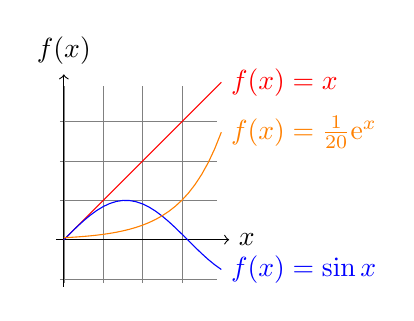
\begin{tikzpicture}[domain=0:4, scale = 0.5]
    \draw[very thin,color=gray] (-0.1,-1.1) grid (3.9,3.9);
  
    \draw[->] (-0.2,0) -- (4.2,0) node[right] {$x$};
    \draw[->] (0,-1.2) -- (0,4.2) node[above] {$f(x)$};
  
    \draw[color=red]    plot (\x,\x)             node[right] {$f(x) =x$};
    % \x r means to convert '\x' from degrees to _r_adians:
    \draw[color=blue]   plot (\x,{sin(\x r)})    node[right] {$f(x) = \sin x$};
    \draw[color=orange] plot (\x,{0.05*exp(\x)}) node[right] {$f(x) = \frac{1}{20} \mathrm e^x$};
\end{tikzpicture}
                \caption{Graphique avec des fonctions}
            \end{figure}
            
        \end{column}
        \begin{column}{0.45\textwidth}
            \begin{figure}[h]
                \centering
                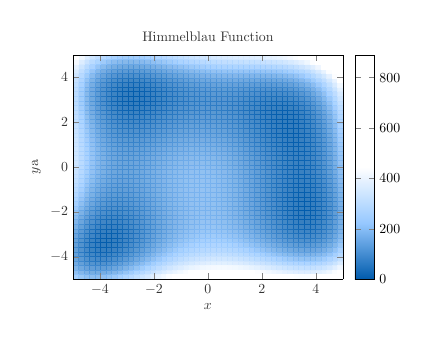
\begin{tikzpicture}[scale = 0.5]
    \begin{axis}[
        colormap={pastel}{ rgb255=(0,91,172) rgb255=(150,200,255) rgb255=(255,255,255)rgb255=(255,255,255)rgb255=(255,255,255)} ,
        view={0}{90},    % Top-down view
        enlargelimits=false,
        axis on top,
        colorbar,        % Add a colorbar
        xlabel=$x$, ylabel=$y$a,
        title={Himmelblau Function},    
        fill opacity=0.8    
    ]
    \addplot3[surf,shader=flat,z buffer=sort,samples=50,domain=-5:5] 
        { (x^2 + y - 11)^2 + (x + y^2 - 7)^2 };
    \end{axis}
\end{tikzpicture}
                \caption{Heatmap pour une fonction prenant 2 dimensions comme argument}
            \end{figure} 
            
        \end{column}
    \end{columns}
\end{frame}

